\documentclass{exam}
\usepackage{amsmath}
\usepackage{url}
\usepackage{tikz}


\newcommand\N{\mathbf{N}}
\newcommand\Z{\mathbf{Z}}
\newcommand\E{\mathbf{E}}
\renewcommand\O{\mathbf{O}}
\newcommand\Q{\mathbf{Q}}
\renewcommand\P{\mathbf{P}}
\def\land{\wedge}
\def\lor{\vee}
\def\xor{\oplus}
\def\T{\top}
\def\F{\bot}
\def\lnot{\neg}

\title{CS250 homeowrk 6}
\author{name: Austen Nelson}
\date{Due: 8/13/19}

\begin{document}
\maketitle

\begin{questions}

\question
Compute the following summations
    \begin{parts}
        \part $\sum_{i=1}^n 6 = 6n$
        \part $\sum_{i=1}^n 5i = \frac{5n(n+1)}{2}$
        \part $\sum_{i=1}^n 3i+2+2^i = \frac{3n(n+1)}{2} + 2n + 2^{n-1} - 2$
        \part $\sum_{i=1}^n 3^i = \frac{3^{n-1} - 3}{2}$
        \part $\sum_{i=1}^n \frac{1}{3^i} - \sum_{i=1}^n \frac{1}{3^{i+1}} = \frac{1}{3} - \frac{1}{3^{n+1}}$
        \part $\sum_{i=1}^n \sum_{j=1}^n j + ij = \sum_{j=1}^{n} jn + \frac{jn(n+1)}{2} = \frac{n^2(n+1)}{2} + \left(\frac{n(n+1)}{2}\right)^2$
        \part $\sum_{k=0}^n \binom{n}{k} 2^k = 3^n$
    \end{parts}

\question
    \begin{parts}
        \part you have 10 people, how many ways are there to split into two teams of 5?
        $$ \binom{10}{5} $$
        \part If you have a red die and green die, there are 6 different ways to roll a 7.
        \part How many ways are there to draw 5 cards from a deck of 52?
        $$ \binom{52}{5} $$

        \part How many possible full house hands are there in poker?
        $$ 12 * 13 = 156 \text{ combinations of values} $$
        $$ \binom{4}{3} \text{ ways to choose the suits for the triple}$$
        $$ \binom{4}{2} \text{ ways to choose the suits for the pair} $$
        $$ 156 * 4 * 6 = 3744 $$

        \part Out of a bag of red, blue and green marbles, how many ways are there to draw three marbles where the order doesn't matter?\\ \\
         3 equivilence classes: All same, all different, 2 are same. \\
         There are 3 ways for all the same, and 1 way for all different. When two are the same, it could be any of the three colors for the pair and there are 2 options left for the remaining marble. \\
         $$ 3 + 1 + 3(2) = 10$$
    \end{parts}

    \pagebreak
\question
There are 38 people in this class. Prove that at least 4 people were born in the same month.\\
   There are 12 months in a year. If there were 3 people born in each month, you would have 36 people. By the pigeon hole principle(38 people, 36 birthmonths), there must be at least one month with 4 or more birthdays.
\question
A round robin tournament is one in which every team players every other team.
Assuming that there are no ties, and every team wins at least one game, prove that two teams won the same number of games. \\
Let n be the number of teams in the tournament. \\
A team can win up to n-1 games (undefeated) \\
   No team can lose all games. So there are n-1 different number of wins for any team. (cardinality of the set of the possible number of wins \{1, 2,...,n-1\} is n-1) \\
By the pigeon hole principle, with n teams and n-1 possible number of wins, at least 2 teams have the same number of wins.
\question
We saw a lot of summation properties in class.\\
Fortunately we don't need to prove all of them separately.
We can prove several of them at the same time.
Use induction to prove that summations are linear:
    $$\sum_{i=m}^n c\cdot a_i + d\cdot b_i = c\cdot \sum_{i=m}^n a_i + d \cdot \sum_{i=m}^n b_i$$
    \begin{align*}
       m = 0, \quad n = 0, \quad c\cdot a_0+d\cdot b_0 = c\cdot a_0+d\cdot b_0 && \text{base case} \\
       \sum_{i=m}^k c\cdot a_i + d\cdot b_i = c\cdot \sum_{i=m}^k a_i + d \cdot \sum_{i=m}^k b_i && \text{inductive hypothesis} \\
       \sum_{i=m}^{k+1} c\cdot a_i + d\cdot b_i  && \text{inductive case} \\
       = \left(c\cdot \sum_{i=m}^k a_i\right) + \left(d \cdot \sum_{i=m}^k b_i\right) + (c \cdot a_{k+1} + d \cdot b_{k+1}) && \text{peel and substitute}\\
       = c\cdot \sum_{i=m}^{k+1} a_i + d \cdot \sum_{i=m}^{k+1} b_i && \text{factor out c and d and combine into sum}
    \end{align*}

\question

\begin{parts}

    \part
How many paths are there from $A$ to $B$ in the following grid
if we're only allowed to move right and down. \\
Assuming one travels on the lines and not from box to box... \\
There are 35 paths from $A$ to $B$

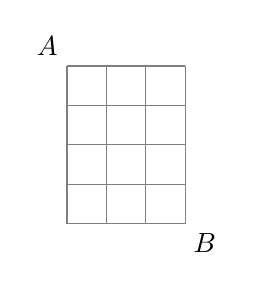
\begin{tikzpicture}
\draw[step=0.5cm,color=gray] (0,0) grid (1.5,2);
\node at (-.25,2.25) {$A$};
\node at (1.75,-.25) {$B$};
\end{tikzpicture}

    \part
Now we have a much larger grid.
This would be very difficult to count the paths by hand.
Instead, let's try to come up with a recursive solution.
Let's have the number of paths from $A$ to $B$ be $P$,
the number of paths from $A$ to $B_1$ be $P_1$, and
the number of paths from $A$ to $B_2$ be $P_2$.
Now give a formula for $P$ in terms of $P_1$ and $P_2$

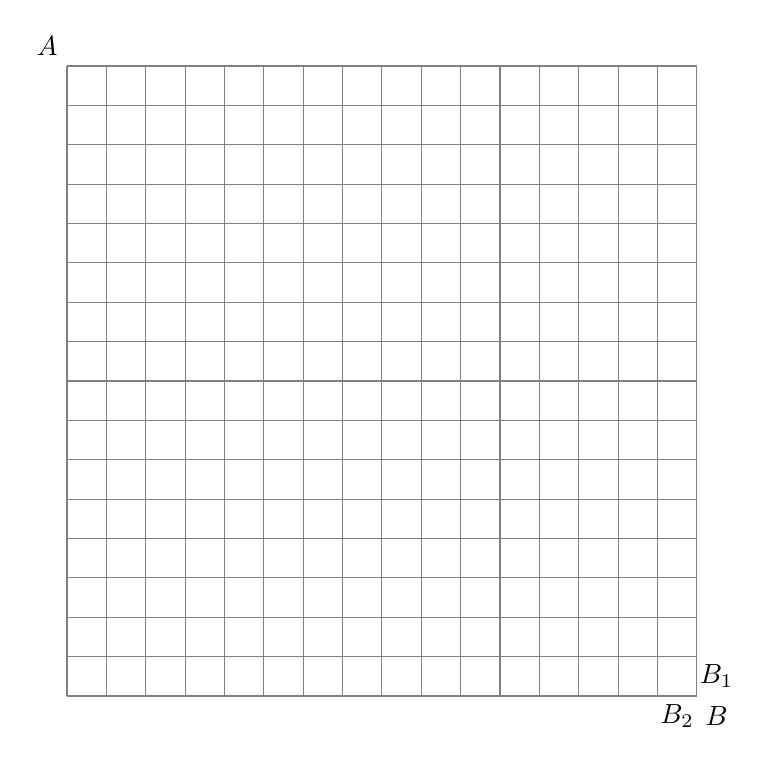
\begin{tikzpicture}
\draw[step=0.5cm,color=gray] (0,0) grid (8,8);
\node at (-.25,8.25) {$A$};
\node at (8.25,.25) {$B_1$};
\node at (7.75,-.25) {$B_2$};
\node at (8.25,-.25) {$B$};
\end{tikzpicture}

$P = P_1 + P_2$\\

    \part
    Now given a grid of $r$ rows and $c$ columns, give a recursive formula for the number of paths from $A$ to $B$\\
    $P(r,c) = P(r-1, c) + P(r, c-1)$\\
    Base cases: $P(1,n) = 1, \quad P(n,1) = 1$ \\

    Hey its Pascal's triangle... nonrecursive: $P(r,c) = \binom{r+c-2}{r-1}$
\end{parts}

\question
I want to answer a simple question from class.
If I roll n dice, how many possible rolls are there when order doesn't matter?
We saw in class that if I have 2 dice, the answer is 21.  Let's generalize this.

First Let's start by calculating the number of ways of rolling 3 dice.
\begin{parts}

\part 
How many ways are to roll 3 dice where all numbers are distinct?\\
   $$\binom{6}{3}$$
\part 
How many ways are to roll 3 dice two dice have the same value?\\
While the order of the dice doesn't matter, the number that rolled twice does.\\
   $$2 \cdot \binom{6}{2}$$
\part 
How many ways are to roll 3 dice all dice are the same?\\
   $$\binom{6}{1}$$
This way of counting dice seems like a good start, but it seems like it could get complicated pretty quickly.
We'll need to break it down.
Notice that in the last part we had 3 cases: all 3 numbers are distinct, 2 numbers are distinct, and only 1 number is distinct.
So, we should really ask the smaller question ``how many ways are there to roll $n$ dice, where $k$ dice are distinct?''

We can again break this into 2 questions.

\part 
How many ways are there to choose the $k$ values for the $n$ dice?\\
   $$\binom{6}{k}$$
For the second question we need to how we group the dice of the same value.
This doesn't seem like a big deal with 3 dice, but let's look at what happens when we have 5.
If I roll 5 dice and get 2 distinct values (4 and 1 for example), how many ways can I break that up?\\
I could have (1 1 1 1 4), (1 1 1 4 4), (1 1 4 4 4), or (1 4 4 4 4).
So there are 4 possible ways.

This gets more complicated with 3 distinct values, so we need a better way to solve the problem.
I could also write this as I have $m_1$ 1s and $m_2$ 4s.
I'll call this the multiplicity of a value.
So the multiplicity of 1 is $m_1$.
The problem is really asking how many different ways can $m_1 + m_2 = 5$.
This is good, because it generalizes.
If I have 3 distinct values, then I'm asking how many ways can $m_1 + m_2 + m_3 = 5$.

\part How many ways are there to assign multiplicities to a roll of $n$ dice with $k$ distinct values? \\
Using stars and bars: 
   $$\binom{n-1}{k-1}$$
Now we can put the last two parts together.
\part How many ways are there to roll $n$ dice with $k$ distinct values?\\
   $$\binom{n-1}{k-1} \cdot \binom{6}{k}$$
\part Give a summation for the number of ways to roll $n$ dice where order doesn't matter.
   $$\sum_{k=1}^{6} \binom{n-1}{k-1} \binom{6}{k}$$

\pagebreak
Ok, that was ... something. I'm kind of concerned about that answer though.
What we really need is a way to check the problem.
We can do that by solving the problem again, but in a different way.
This time we're going to take our roll and sort it.\\
So if I roll 7 dice (4 3 4 1 6 2 2), I'll get (1 2 2 3 4 4 6)
If two rolls sort to the same thing, then they're the same roll.

Now that I have the numbers grouped together, this looks like a good spot for stars and bars.
In This case a I'll put a star every time there's a number, and a bar every time a number goes up by 1.
So the roll (1 2 2 3 4 4 6) will be (* $|$ * * $|$ * $|$ * * $|$ $|$ *).
Since I didn't use the number 5, I have 2 bars in a row.
I'll always have $n$ stars, and $5$ bars.

\part use this stars and bars set up to get a new formula for the number of ways to roll $n$ dice where order doesn't matter.
   $$\binom{n+5}{5}$$

\part Finally, use the recursive formula ${n \choose k} = {n-1 \choose k} + {n-1 \choose k-1}$
to show that part g and part h are really the same. \\
\begin{align*}
   \sum_{k=1}^{6} \binom{n-1}{k-1} \binom{6}{k}& \\
   &= 6\binom{n-1}{0} + 15\binom{n-1}{1} + 20\binom{n-1}{2} + 15\binom{n-1}{3} + 6\binom{n-1}{4} + \binom{n-1}{5} \\
   \binom{n+5}{5} &\\
   &=\binom{n+4}{5} + \binom{n+4}{4}\\
   &=\binom{n+3}{5} + 2\binom{n+3}{4} + \binom{n+3}{3}\\
   &=\binom{n+2}{5} + 3\binom{n+2}{4} + 3\binom{n+2}{3} + \binom{n+2}{2}\\
   &=\binom{n+1}{5} + 4\binom{n+1}{4} + 6\binom{n+1}{3} + 4\binom{n+1}{2} + \binom{n+1}{1}\\
   &=\binom{n}{5} + 5\binom{n}{4} + 10\binom{n}{3} + 10\binom{n}{2} + 5\binom{n}{1} + \binom{n}{0}\\
   &=\binom{n-1}{5} + 6\binom{n-1}{4} + 15\binom{n-1}{3} + 20\binom{n-1}{2} + 15\binom{n-1}{1} + 6\binom{n-1}{0}
\end{align*}
\end{parts}

\end{questions}
\end{document}
